\documentclass[12pt,a4paper]{amsart}

\usepackage[T1]{fontenc}
\usepackage[utf8]{inputenc}
\usepackage[british]{babel}
\usepackage{mathtools}
\usepackage{amsthm}
\usepackage{amssymb}
\usepackage{mathrsfs}
\usepackage{enumitem}
\usepackage{tikz-cd}
\usetikzlibrary{decorations.markings}
\usepackage{float}
\usepackage{hyperref}
\urlstyle{same}
\usepackage[noabbrev]{cleveref}

\theoremstyle{plain}
\newtheorem{thm}{Theorem}[section]
\newtheorem*{thm*}{Theorem}
\newtheorem{lm}[thm]{Lemma}
\newtheorem{prop}[thm]{Proposition}
\newtheorem{cor}[thm]{Corollary}
\theoremstyle{definition}
\newtheorem{defn}[thm]{Definition}
\newtheorem{exmp}[thm]{Example}
\newtheorem{xca}[thm]{Exercise}
\theoremstyle{remark}
\newtheorem{rem}[thm]{Remark}
\Crefname{thm}{Theorem}{Theorems}
\Crefname{lm}{Lemma}{Lemmas}
\Crefname{prop}{Proposition}{Propositions}
\Crefname{cor}{Corollary}{Corollaries}
\Crefname{defn}{Definition}{Definitions}
\Crefname{exmp}{Example}{Examples}
\Crefname{xca}{Exercise}{Exercises}
\Crefname{rem}{Remark}{Remarks}

\title[Talk on Hilbert schemes of points on surfaces]{Talk on Hilbert schemes of points on surfaces}
\author[Pedro N\'{u}\~{n}ez]{Pedro N\'{u}\~{n}ez}
\address{Pedro N\'{u}\~{n}ez \newline
\indent Albert-Ludwigs-Universit\"{a}t Freiburg, Mathematisches Institut \newline
\indent Ernst-Zermelo-Straße 1, 79104 Freiburg im Breisgau (Germany)}
\email{\normalfont\href{mailto:pedro.nunez@math.uni-freiburg.de}{pedro.nunez@math.uni-freiburg.de}}
\renewcommand*{\urladdrname}{\itshape Homepage}
\urladdr{\normalfont\href{https://home.mathematik.uni-freiburg.de/nunez/}{https://home.mathematik.uni-freiburg.de/nunez}}
\thanks{The author gratefully acknowledges support by the DFG-Graduiertenkolleg GK1821 ``Cohomological Methods in Geometry'' at the University of Freiburg.}
\date{\today}

\setcounter{tocdepth}{1}
\sloppy
\makeatletter
\hypersetup{
  pdfauthor={\authors},
  pdftitle={\@title},
  colorlinks,
  linkcolor=[rgb]{0.2,0.2,0.6},
  citecolor=[rgb]{0.2,0.6,0.2},
  urlcolor=[rgb]{0.6,0.2,0.2}}
\makeatother

\begin{document}

\maketitle

\begin{abstract}
  Script for the 7\textsuperscript{th} talk of the seminar on Heisenberg algebras and Hilbert schemes of points on surfaces organized by Mara Ungureanu during the Summer Term 2021 at the University of Freiburg.
\end{abstract}

\tableofcontents

\begin{center}
  \textcolor{gray}{---parts in gray will be omitted during the talk---}
\end{center}

\setcounter{section}{-1}

\section{Conventions and notation}

We always work over $\mathbb{C}$.
By a variety we mean an integral separated scheme of finite type over $\mathbb{C}$ as in \cite{har77}.

The main references for the talk are \cite[\S 1]{nak99} and the notes in \url{http://www.math.utah.edu/~filipazz/seminar_notes/fall_2016/Hilbert_scheme_points.pdf}.

\section{Introduction}

We would like to parametrize unordered tuples of $n$-points on a smooth projective surface $X$.
Consider the $n$-fold product $X \times \cdots \times X$ of $X$ with itself.
This gives us ordered tuples with potential repetitions.
To avoid repetitions we can remove the closed subset of all tuples with at least two equal points; this gives us a dense open subset of the product.
To forget about the order of the tuples we may quotient out by the action of the symmetric group $\mathfrak{S}_{n}$ permuting the factors.
This gives us a smooth variety parametrizing unordered tuples of $n$-points on $X$, but we would now like to compactify this parameter space.

A natural candidate would be the quotient of the whole $n$-fold product $X \times \cdots \times X$ by the $\mathfrak{S}_{n}$ action permuting the factors, which is called the $n$-th symmetric power of $X$, denoted $S^{n}X$.
But $S^{n}X$ has singularities, so instead we look at the Hilbert scheme of $n$-points on $X$, denoted $X^{[n]}$.
We will see that there is a morphism $\pi \colon X^{[n]} \to S^{n}X$, called the \textit{Hilbert--Chow} morphism, which is a resolution of singularities.

\section{Symmetric products and their stratification}

\begin{defn}[Symmetric powers]
  Let $X$ be a quasi-projective variety and let $n \in \mathbb{N}_{>0}$.
  Let $\mathfrak{S}_{n}$ denote the symmetric group of order $n$.
  We define the \textit{$n$-th symmetric power of $X$}, denoted $S^{n}X$, to be the quotient of the $n$-fold product $X \times \cdots \times X$ with itself by the action of $\mathfrak{S}_{n}$ which permutes the factors.
\end{defn}

\begin{rem}
  Quotients of varieties by algebraic actions of finite groups are discussed in \Cref{sec:quotient}.
  It is shown in \Cref{thm:quotient} that the quotient $S^{n}X$ exists as a scheme and is in fact a quasi-projective variety.
  The fibers of the quotient morphism over closed points are precisely the orbits of closed points in $X$, and the quotient space carries the quotient topology induced by the quotient morphism.
  Moreover, let $\mathbf{P}$ be any of the following properties:
  \begin{itemize}
    \item affine,
    \item projective,
    \item normal.
  \end{itemize}
  If $X$ is $\mathbf{P}$, then $S^{n}X$ is $\mathbf{P}$.
  In particular, $S^{n}X$ is a normal projective variety if $X$ was a smooth projective variety.
\end{rem}

\begin{exmp}
  Let $n \in \mathbb{N}_{>0}$.
  Then $S^{n}(\mathbb{A}^{1}) \cong \mathbb{A}^{n}$.
  Indeed, it follows from \Cref{cor:affinequotient} that
  \[ S^{n}(\mathbb{A}^{1}) = \operatorname{Spec}\left(\mathbb{C}[x_{1}, \ldots, x_{n}]^{\mathfrak{S}_{n}}\right), \]
  so the claim follows from the \href{https://en.wikipedia.org/wiki/Elementary_symmetric_polynomial#Fundamental_theorem_of_symmetric_polynomials}{fundamental theorem of symmetric polynomials}.
\end{exmp}

In order to show later that the yet-to-be-defined Hilbert--Chow morphism $\pi \colon X^{[n]} \to S^{n}X$ is a resolution of singularities in the case of surfaces, it will be convenient to consider the following stratification of $S^{n}X$.
Let $k \in \mathbb{N}_{>0}$ such that $k \leq n$.
Consider a tuple $\nu = (\nu_{1}, \ldots, \nu_{k})$ be with $\nu_{1} \geq \nu_{2} \geq \ldots \geq \nu_{k} > 0$ such that $n = \nu_{1} + \ldots + \nu_{k}$.
Call this a \textit{partition of $n$} of \textit{length} $l(\nu) := k$.
Then, for each partition $\nu$ of $n$, we define
\[ S^{n}_{\nu}X := \left\{ \quad \sum_{i = 1}^{k} \nu_{i}[x_{i}] \in S^{n}X \quad \middle| \quad x_{i} \neq x_{j} \text{ for } i \neq j \quad \right\}. \]

\color{red} This is a stratification of $S^{n}X$ \color{black} and \color{red} $\dim(S^{n}_{\nu}X) = l(\nu)\dim(X)$\color{black}.
Moreover, the \color{red} open \color{black} stratum $S^{n}_{(1,\ldots,1)}X$ is smooth if $X$ is smooth, because \color{red} the quotient by a free action of a finite group on a smooth variety is smooth\color{black}.

\section{Hilbert--Chow morphism}

\begin{prop}
  Let $X$ be a quasi-projective surface and let $n \in \mathbb{N}_{>0}$.
  Let $X^{[n]}$ be the Hilbert scheme of $n$-points on $X$ and let $S^{n}X$ be the $n$-th symmetric power of $X$.
  Then the set-theoretic morphism defined on closed points as
  \begin{align*}
    \pi \colon X^{[n]} & \longrightarrow S^{n}X \\
    [Z] & \longmapsto \sum_{x \in X} \dim_{\mathbb{C}}(\mathscr{O}_{Z,x})[x] 
  \end{align*}
  defines a $\mathbb{C}$-scheme morphism called the \textit{Hilbert--Chow morphism}.

  \begin{proof}
    We follow the proof in \cite[\S 3.2]{leh00}.
    Let $f \in X^{[n]}(T)$and let $\mathcal{Z}$ be the corresponding family over $T$, i.e.~$\mathcal{Z} \subseteq T \times X$ and the restriction of the projection $\mathcal{Z} \to T$ is a finite flat morphism of degree $n$.
    Let $t_{0} \in T$ be a closed point, which corresponds to a 
  \end{proof}
\end{prop}

\section{Case of curves}

\section{Hilbert scheme of points on a surface}

\appendix

\section{Quotients of quasi-projective varieties by finite groups}\label{sec:quotient}

We will mostly follow the notes in \url{http://www.math.lsa.umich.edu/~mmustata/appendix.pdf} in this appendix.

\begin{rem}
  Let $G$ be a finite group and let $X = \operatorname{Spec}{A}$ be an affine variety.
  An action of $G$ on $A$ by $\mathbb{C}$-algebra automorphisms \textit{from the left} is the same as an aciton of $G$ on $X$ by $\mathbb{C}$-scheme morphisms \textit{from the right}.
  The two things are more explicitly related as follows:
  \[ (g \cdot f)(x) = f(x \cdot g). \]
\end{rem}

From now on, by an \textit{action} of a finite group $G$ on a $\mathbb{C}$-scheme (resp.~on a $\mathbb{C}$-algebra) we will always mean a right action via $\mathbb{C}$-algebra morphisms (resp.~a left action via $\mathbb{C}$-scheme morphisms).
There are various notions of quotients in algebraic geometry, cf.~\cite[\S 0.1]{mfk94}.
Fortunately, in the case of finite groups, the various notions agree.

\begin{defn}[Categorical quotient]
  Let $\sigma \colon X \times G \to X$ be an action of a finite group $G$ on a $\mathbb{C}$-scheme $X$.
  A \textit{categorical quotient} of $X$ by $G$ is a pair $(Y,\pi)$ consisting of a $\mathbb{C}$-scheme $Y$ and a $\mathbb{C}$-scheme morphism $\pi \colon X \to Y$ with the following properties:
  \begin{enumerate}[label=\roman*)]
    \item $\pi$ is $G$-invariant, i.e.~we have $\pi \circ \sigma = \pi \circ p_{1}$, where $p_{1} \colon X \times G \to X$ is the projection.
    \item $\pi$ is universal with respect to the property in $i)$, i.e.~for every pair $(Z,\psi)$ consisting of a $\mathbb{C}$-scheme $Z$ and a $G$-invariant $\mathbb{C}$-scheme morphism $\psi \colon X \to Z$, there exists a unique $\mathbb{C}$-scheme morphism $\bar{\psi} \colon Y \to Z$ such that $\bar{\psi} \circ \pi = \psi$.
  \end{enumerate}
\end{defn}

\begin{lm}\label{lm:uniquequotient}
  Let $\sigma \colon X \times G \to X$ be an action of a finite group $G$ on a $\mathbb{C}$-scheme $X$.
  If a categorical quotient $(Y,\pi)$ exists, it is unique up to unique isomorphism.
  That is, if $(Y', \pi')$ is another categorical quotient, then there exists a unique $\mathbb{C}$-scheme isomorphism $\bar{\pi}' \colon Y \to Y'$ such that $\pi' = \bar{\pi}' \circ \pi$.
  
  \begin{proof}
    Since the pair $(Y', \pi')$ satisfies the property $i)$ above, the universal property of $(Y, \pi)$ ensures the existence of a $\mathbb{C}$-scheme morphism $\bar{\pi}' \colon Y \to Y'$ such that $\pi' = \bar{\pi}' \circ \pi$.
    It remains to show that this is an isomorphism.
    The roles of $(Y, \pi)$ and $(Y', \pi')$ are symmetric, so we can also find a $\mathbb{C}$-scheme morphism $\bar{\pi} \colon Y' \to Y$ making the following diagram commute:

    \begin{center}
      \begin{tikzcd}
        & & X \arrow[bend right=30]{dll}{\pi'} \arrow{dl}{\pi} \arrow{dr}{\pi'} \arrow[bend left=30]{drr}{\pi} & & \\
        Y' \arrow{r}{\bar{\pi}} & Y \arrow{rr}{\bar{\pi}'} & & Y' \arrow{r}{\bar{\pi}} & Y
      \end{tikzcd}
    \end{center}

    The uniqueness part of the universal property in $ii)$ above ensures that $\bar{\pi} \circ \bar{\pi}' = \operatorname{id}_{Y}$ and $\bar{\pi}' \circ \bar{\pi} = \operatorname{id}_{Y'}$, so $\bar{\pi}'$ is indeed a $\mathbb{C}$-scheme isomorphism.

  \end{proof}
\end{lm}

\begin{rem}
  In view of the uniqueness given by \Cref{lm:uniquequotient}, we will sometimes denote a categorical quotient by $(X/G, \pi)$.
\end{rem}

\begin{defn}[Geometric quotient]
  Let $\sigma \colon X \times G \to X$ be an action of a finite group $G$ on a finite type\footnote{This assumption makes condition $(2)$ below less cumbersome to formulate, cf.~\cite[Definition 0.6]{mfk94}.} $\mathbb{C}$-scheme $X$.
  A \textit{geometric quotient} of $X$ by $G$ is a pair $(Y, \pi)$ consisting of a $\mathbb{C}$-scheme $Y$ and a $\mathbb{C}$-scheme morphism $\pi \colon X \to Y$ with the following properties:
  \begin{enumerate}
    \item $\pi$ is $G$-invariant, i.e.~property $i)$ above holds.
    \item $\pi$ is surjective and the fibers of $\pi$ over closed points of $Y$ are precisely the orbits of the closed points of $X$.
    \item $Y$ carries the quotient topology induced by $\pi$, i.e.~a subset $V \subseteq Y$ is open if and only if $\pi^{-1}(V) \subseteq X$ is open.
    \item The structure sheaf $\mathscr{O}_{Y}$ is the subsheaf of $\pi_{*}\mathscr{O}_{X}$ consisting of $G$-invariant functions, i.e.~if $f \in \Gamma(V, \pi_{*}\mathscr{O}_{X}) = \Gamma(\pi^{-1}(V),\mathscr{O}_{X})$, then $f \in \Gamma(V, \mathscr{O}_{Y})$ if and only if

      \begin{center}
        \begin{tikzcd}
          \pi^{-1}(V) \times G \arrow{r}{\sigma} \arrow{d}{p_{1}} & \pi^{-1}(V) \arrow{d}{f} \\
          \pi^{-1}(V) \arrow{r}{f} & \mathbb{A}^{1}
        \end{tikzcd}
      \end{center}
      commutes, where we regard the regular function$f$ as a $\mathbb{C}$-scheme morphism $f \colon \pi^{-1}(V) \to \mathbb{A}^{1}$.
    \end{enumerate}
\end{defn}

\begin{rem}\label{rem:loct}
  Being a geometric quotient is local on the target in the sense of \cite[Appendix C]{gw10}.
\end{rem}

\begin{prop}
  Let $\sigma \colon X \times G \to X$ be an action of a finite group $G$ on a finite type $\mathbb{C}$-scheme $X$ and let $(Y, \pi)$ be a geometric quotient of $X$ by $G$.
  Then $(Y, \pi)$ is also a categorical quotient.

  \begin{proof}
    We follow the proof given in \cite[Proposition 0.1]{mfk94}.
    Suppose we are given another pair $(Z, \psi)$ with the property $i)$ above, i.e.~such that $\psi \colon X \to Z$ is a $G$-invariant $\mathbb{C}$-scheme morphism.
    Recall from \cite[Exercise II.2.4]{har77} that if $Z = \operatorname{Spec}(B)$ was affine, then $\mathbb{C}$-scheme morphisms $Y \to Z$ correspond bijectively to $\mathbb{C}$-algebra morphisms $B \to \Gamma(Y,\mathscr{O}_{Y})$.
    The idea is to use this combined with our understanding of $\Gamma(Y,\mathscr{O}_{Y})$ given by property $(4)$ above.

    So let $\{ W_{i} \}_{i \in I}$ be an affine open cover of $Z$, say $W_{i} = \operatorname{Spec}(B_{i})$ for each $i \in I$.
    Since $\psi$ is $G$-invariant, each $U_{i} := \psi^{-1}(W_{i})$ is an invariant open subset in $X$.
    Therefore $\pi^{-1}(\pi(\psi^{-1}(W_{i}))) = \psi^{-1}(W_{i})$.
    Let us call $V_{i} := \pi(\psi^{-1}(W_{i}))$ for each $i \in I$.
    Since $Y$ carries the quotient topology induced by $\pi$ and $\pi^{-1}(V_{i}) = \psi^{-1}(W_{i})$ is open in $X$, we deduce that $V_{i}$ is also open in $Y$ for each $i \in I$.
    Surjectivity of $\pi$ ensures that $\{ V_{i} \}_{i \in I}$ is an open cover of $Y$.

    As usual with existence and uniqueness statements, it will be convenient to start by arguing the uniqueness, which will then likely give us some hints as to how to show the existence.
    Suppose that the desired factorization $\bar{\psi} \colon Y \to Z$ existed.
    Then, since $\psi = \bar{\psi} \circ \pi$, we have
    \[ \bar{\psi}(V_{i}) = \bar{\psi}(\pi(\psi^{-1}(W_{i}))) = \psi(\psi^{-1}(W_{i})) \subseteq W_{i} \]
    for each $i \in I$.
    So for each $i \in I$, our factorization $\bar{\psi} \colon Y \to Z$ would yield a morphism $\bar{\psi}_{i} \colon V_{i} \to W_{i}$ such that $\psi_{i} = \bar{\psi}_{i} \circ \pi_{i}$, where by $\pi_{i} \colon U_{i} \to V_{i}$ and $\psi_{i} \colon U_{i} \to W_{i}$ are the morphisms induced by $\pi$ and $\psi$ respectively.
    Since the target $W_{i} = \operatorname{Spec}(B_{i})$ of $\bar{\psi}_{i}$ is affine, \cite[Exercise II.2.4]{har77} tells us that $\bar{\psi}_{i}$ is uniquely determined by the correspdonding morphism of $\mathbb{C}$-algberas $h_{i} \colon B_{i} \to \Gamma(V_{i}, \mathscr{O}_{Y})$.
    Commutativity of the triangle of $\mathbb{C}$-schemes
    
    \begin{center}
      \begin{tikzcd}
        U_{i} \arrow{r}{\psi_{i}} \arrow{d}{\pi_{i}} & W_{i} \\
        V_{i} \arrow[swap]{ur}{\bar{\psi}_{i}} & 
      \end{tikzcd}
    \end{center}
    translates into commutativity of the triangle of $\mathbb{C}$-algebras

    \begin{center}
      \begin{tikzcd}
        \Gamma(U_{i}, \mathscr{O}_{X}) & B_{i} \arrow[swap]{l}{\psi^{*}_{i}} \arrow{dl}{h_{i}} \\
        \Gamma(V_{i}, \mathscr{O}_{Y}) \arrow{u}{\pi^{*}_{i}} & 
      \end{tikzcd}
    \end{center}

    But property $(4)$ above tells us that $\pi_{i}^{*}$ is the inclusion of the $G$-invariant regular functions on $U_{i}$, in particular an injective $\mathbb{C}$-algebra morphism.
    So each $h_{i}$ is uniquely determined by $\psi$, hence so is each $\bar{\psi}_{i}$ and hence so is $\bar{\psi}$ itself.

    Now to show existence the plan is first to show existence of the $h_{i}$ defined as above, and then check that the corresponding $\bar{\psi}_{i}$ glue together into a $\mathbb{C}$-scheme morphism $Y \to Z$.
    So let $i \in I$ and let us show that $h_{i}$ exists, i.e.~let us show that the image of $\psi_{i}^{*}$ consists of $G$-invariant regular functions on $U_{i}$.
    Let then $b \in B_{i}$ be a regular function on $W_{i}$, which we regard as a $\mathbb{C}$-scheme morphism $b \colon W_{i} \to \mathbb{A}^{1}$.
    The $G$-invariance assumption on $\psi$ translates into saying that $\psi_{i}(x \cdot g) = \psi_{i}(x)$ for each closed point $x \in U_{i}$ and each $g \in G$.
    We want to show that $g \cdot \psi_{i}^{*}(b) = \psi_{i}^{*}(b)$ for each $g \in G$, so let $g \in G$ be arbitrary.
    We regard again regular functions as $\mathbb{C}$-scheme morphisms into $\mathbb{A}^{1}$ and check the equality on closed points of $U_{i}$:

    \begin{align*}
      (g \cdot \psi_{i}^{*}(b))(x) & = \psi_{i}^{*}(b)(x \cdot g) \\
      & = b(\psi_{i}(x \cdot g)) \\
      & = b(\psi_{i}(x)) \\
      & = (\psi_{i}^{*}(b))(x).
    \end{align*}
    Hence the image of $\psi_{i}^{*}$ lies in the subalgebra of $G$-invariant regular functions on $U_{i}$, and thus we can find the desired factorization $h_{i}$.

    The previous argument gives us a factorization $\bar{\psi}_{i} \colon V_{i} \to W_{i}$ for each $i \in I$, and it remains to show that these glue together into a morphism $\bar{\psi} \colon Y \to Z$.
    Given $i, j \in I$, both $\bar{\psi}_{i}|_{V_{i} \cap V_{j}} \colon V_{i} \cap V_{j} \to W_{i}$ and $\bar{\psi}_{j}|_{V_{i} \cap V_{j}} \colon V_{i} \cap V_{j} \to W_{i}$ are uniquely determined by the correpsonding $\mathbb{C}$-algebra morphisms $h_{ij} , h_{ji} \colon B_{i} \to \Gamma(V_{i} \cap V_{j}, \mathscr{O}_{Y})$.
    The arguments above show that we must have $h_{ij} = h_{ji}$, so the two morphisms agree on the intersections and we can glue them together as we wanted.

  \end{proof}
\end{prop}

\begin{lm}\label{lm:finitetype}
  Let $G$ be a finite group.
  Let $A$ be a finite type $\mathbb{C}$-algebra and assume that the group $G$ acts on $A$ from the left by $\mathbb{C}$-algebra automorphisms.
  Then the set of invariant elements $A^{G}$ is a $\mathbb{C}$-subalgebra of $A$ which is of finite type over $\mathbb{C}$.

  \begin{proof}
    Let $\rho \colon G \to \operatorname{Aut}_{\mathbb{C}}(A)$ be the given left action.
    Let us first quickly ensure that
    \[ A^{G} := \bigcap_{g \in G} \{ a \in A \mid \rho(g)(a) = a \} \]
    is a $\mathbb{C}$-subalgebra of $A$.
    \begin{itemize}
      \item $A^{G} \subseteq A$ is a subgroup.
        Indeed, since $\rho(g)$ is a ring morphism for every $g \in G$, we have $0 \in A^{G}$.
        And if $a_{1}, a_{2} \in A^{G}$ and $g \in G$, then it follows again from $\rho(g)$ being a ring morphism that
        \[ \rho(g)(a_{1}+a_{2}) = \rho(g)(a_{1}) + \rho(g)(a_{2}) = a_{1} + a_{2}. \]
      \item $A^{G} \subseteq A$ is a subring.
        We have seen already that it is a subgroup.
        Since $\rho(g)$ is a ring morphism for every $g \in G$, we also have $1 \in A^{G}$, so it remains only to show that $A^{G}$ is closed under products.
        If $a_{1}, a_{2} \in A^{G}$ and $g \in G$, then using once again that $\rho(g)$ is a ring morphism we see that
        \[ \rho(g)(a_{1}a_{2}) = \rho(g)(a_{1})\rho(g)(a_{2}) = a_{1}a_{2}. \]
      \item $A^{G} \subseteq A$ is a $\mathbb{C}$-vector subspace.
        We have seen already that it is a subgroup, so it remains only to show that $A^{G}$ is closed under scalar product.
        If $a \in A^{G}$, $\lambda \in \mathbb{C}$ and $g \in G$, then we use the assumption that $\rho(g)$ is $\mathbb{C}$-linear to deduce that
        \[ \rho(g)(\lambda a) = \lambda \rho(g)(a) = \lambda a. \]
    \end{itemize}
    
    The other assertion in the lemma is that $A^{G}$ is a finite type $\mathbb{C}$-algebra.
    The idea is to write $A^{G}$ as a finite $B$-module for some suitable finite type $\mathbb{C}$-algebra $B$.
    Then it would follow that $A^{G}$ is a finite type $\mathbb{C}$-algebra as well.
    Indeed, let $\beta_{1}, \ldots, \beta_{m} \in B$ be generators of $B$ as an algebra over $\mathbb{C}$, and let $e_{1}, \ldots, e_{l} \in A^{G}$ be generators of $A^{G}$ as a $B$-module.
    Then we can write any $a \in A^{G}$ as a $B$-linear combination
    \[ a = \sum_{i = 1}^{l} b_{i}e_{i}, \]
    and in turn each $b_{i}$ as an algebraic combination
    \[ b_{i} = f_{i}(\beta_{1}, \ldots, \beta_{m}) \]
    for some $f_{i} \in \mathbb{C}[\beta_{1}, \ldots, \beta_{m}]$.
    It follows that we can write $a$ as an algebraic combination in the variables $\beta_{1}, \ldots, \beta_{m}, e_{1}, \ldots, e_{l}$, so these elements would form a system of generators of $A^{G}$ as a $\mathbb{C}$-algebra.

    In order to construct such $B$, we first note that the inclusion $A^{G} \subseteq A$ is an integral ring extension.
    Indeed, every $a \in A$ is a root of the monic polynomial
    \[ P_{a}(t) := \prod_{g \in G}(t - \rho(g)(a)), \]
    whose coefficients are in $A^{G}$ by Vieta's formulas.
    Let $\alpha_{1}, \ldots, \alpha_{m} \in A$ be generators of $A$ as an algebra over $\mathbb{C}$.
    Let $\{ c_{i,j} \}_{j = 0}^{d_{i}}$ be the coefficients of $P_{\alpha_{i}}$ for each $i \in \{1, \ldots, m\}$.
    Then define $B$ to be the $\mathbb{C}$-subalgebra of $A$ generated by all these coefficients $\{ c_{1,0}, \ldots, c_{1,d_{1}}, c_{2,0}, \ldots, c_{m,d_{m}} \}$.
    Since each of its generators is contained in $A^{G}$, we see that $B$ is also a $\mathbb{C}$-subalgebra of $A^{G}$.
    Moreover, by construction $B \subseteq A$ is an integral ring extension.
    The elements $\alpha_{1}, \ldots, \alpha_{m}$ still generate $A$ as a $B$-algebra, so $A$ is a finitely generated $B$-module \cite[Corollary 5.2]{am69}.
    But $B$ is noetherian, because it is a finitely generated $\mathbb{C}$-algebra, so every $B$-submodule of $A$ must also be finitely generated as a $B$-module.
    Therefore $A^{G}$ is a finitely generated $B$-module, which as explained earlier concludes the proof.
  \end{proof}

\end{lm}

\begin{lm}\label{lm:finitesurjective}
  In the situation of \Cref{lm:finitetype}, the induced $\mathbb{C}$-scheme morphism $\pi \colon \operatorname{Spec}(A) \to \operatorname{Spec}(A^{G})$ is finite and surjective.

  \begin{proof}
    It follows from the proof of \Cref{lm:finitetype} that $A$ is finitely generated as an $A^{G}$-module, so the induced morphism $\pi$ is finite by definition \cite[p.~84]{har77}.
    Surjectivity follows from \cite[\href{https://stacks.math.columbia.edu/tag/00GQ}{Tag 00GQ}]{stacks-project}.
  \end{proof}
\end{lm}

\begin{rem}\label{rem:irreducible}
  It follows from \Cref{lm:finitesurjective} that $\operatorname{Spec}(A^{G})$ is irreducible if $\operatorname{Spec}(A)$ was irreducible.
  But the converse is not true, e.g.~consider $\mathbb{Z}/2\mathbb{Z}$ acting non-trivially on two points.
\end{rem}

\begin{lm}\label{lm:fibers}
  In the situation of \Cref{lm:finitetype}, the fibers of $\pi$ over closed points of $Y$ are precisely the orbits of the closed points of $X$ under the action of $G$.
  In particular, $\pi$ is $G$-invariant.

  \begin{proof}
    Let $x \in X$ be a closed point.
    Let us check first that the orbit $x \cdot G$ is contained in the fiber $\pi^{-1}(\pi(x))$.
    Let $\mathfrak{m} \subseteq A$ be the maximal ideal corresponding to $x$, i.e.
    \[ \mathfrak{m} = \{ f \in A \mid f(x) = 0 \}. \]
    Let $g \in G$.
    Our goal is to show that $\pi(x) = \pi(x \cdot g)$.
    The maximal ideal corresponding to the point $x \cdot g$ is given by
    \[ \{ f \in A \mid f(x \cdot g) = 0 \} = \{ f \in A \mid (g \cdot f)(x) = 0 \} = \{ g\cdot f \mid f \in \mathfrak{m} \} = g \cdot \mathfrak{m}. \]
    So we need to show that
    \[ \mathfrak{m} \cap A^{G} = (g \cdot \mathfrak{m}) \cap A^{G}. \]
    But we have
    \begin{align*}
      (g \cdot \mathfrak{m}) \cap A^{G} & = \{ (g \cdot f) \in A^{G} \mid f \in \mathfrak{m} \} \\
      & = \{ g^{-1} \cdot (g \cdot f) \in A^{G} \mid f \in \mathfrak{m} \} \\
      & = \{ f \in A^{G} \mid f \in \mathfrak{m} \} \\
      & = \mathfrak{m} \cap A^{G}. 
    \end{align*}
    Hence $x \cdot G \subseteq \pi^{-1}(\pi(x))$.

    Conversely, let $x_{1}, x_{2} \in \pi^{-1}(\pi(x_{1}))$ be closed points with corresponding maximal ideals $\mathfrak{m}_{1}$ and $\mathfrak{m}_{2}$ respectively.
    The assumption that $x_{1}$ and $x_{2}$ are in the same fiber translates into the equality
    \[ \mathfrak{m}_{1} \cap A^{G} = \mathfrak{m}_{2} \cap A^{G}. \]
    We use this equality to show that
    \[ \mathfrak{m}_{1} \subseteq \bigcup_{g \in G} (g \cdot \mathfrak{m}_{2}). \]
    Indeed, given any $f \in \mathfrak{m}_{1}$, we can produce a $G$-invariant element in the maximal ideal by looking at the (finite) product
    \[ \prod_{g \in G} (g \cdot f) \in \mathfrak{m}_{1} \cap A^{G} = \mathfrak{m}_{2} \cap A^{G} \subseteq \mathfrak{m}_{2}. \]
    Since $\mathfrak{m}_{2}$ is a prime ideal, there exists some $g \in G$ such that $g \cdot f \in \mathfrak{m}_{2}$.
    Hence $\mathfrak{m}_{1} \subseteq \cup_{g \in G} (g \cdot \mathfrak{m}_{2})$ as claimed.
    Since $G$ acts by ring morphisms, each ideal $g \cdot \mathfrak{m}_{2}$ is again a prime ideal.
    So we may apply the prime avoidance lemma to conclude that there exists some $g_{1} \in G$ such that $\mathfrak{m}_{1} \subseteq g_{1} \cdot \mathfrak{m}_{2}$.
    By symmetry of $x_{1}$ and $x_{2}$ there exists some $g_{2} \in G$ such that $\mathfrak{m}_{2} \subseteq g_{2} \cdot \mathfrak{m}_{1}$.
    So
    \[ \mathfrak{m}_{1} \subseteq g_{1} \cdot \mathfrak{m}_{2} \subseteq g_{1} g_{2} \cdot \mathfrak{m}_{1}. \]
    Since $G$ acts by ring automorphisms, $\mathfrak{m}_{1}$ and $g_{1} g_{2} \cdot \mathfrak{m}_{1}$ are prime ideals of the same height.
    Therefore $\mathfrak{m}_{1} = g_{1} g_{2} \cdot \mathfrak{m}_{1}$.
    From this we finally deduce that
    \[ g_{1} \cdot \mathfrak{m}_{2} \subseteq g_{1}g_{2} \cdot \mathfrak{m}_{1} = \mathfrak{m}_{1} \subseteq g_{1} \cdot \mathfrak{m}_{2}, \]
    so that $\mathfrak{m}_{1} = g_{1} \cdot \mathfrak{m}_{2}$ and $x_{1} \in x_{2} \cdot G$.
  \end{proof}
\end{lm}

\begin{lm}\label{lm:topology}
  In the situation of \Cref{lm:finitetype}, the topology on $\operatorname{Spec}(A^{G})$ is the quotient topology induced by $\pi$.
  
  \begin{proof}
    We need to show that a subset $U \subseteq \operatorname{Spec}(A^{G})$ is open as soon as $\pi^{-1}(U)$ is open.
    So let $U \subseteq \operatorname{Spec}(A^{G})$ be a subset such that $\pi^{-1}(U)$ is open in $\operatorname{Spec}(A)$.
    Let $Z := \operatorname{Spec}(A^{G}) \setminus U$.
    Then $\pi^{-1}(Z) = \operatorname{Spec}(A) \setminus \pi^{-1}(U)$, which by assumption is a closed subset in $\operatorname{Spec}(A)$.
    By \Cref{lm:finitesurjective} the morphism $\pi$ is surjective, so $Z \subseteq \pi(\pi^{-1}(Z))$.
    And $\pi(\pi^{-1}(Z)) \subseteq Z$ is always true, so we deduce that $\pi(\pi^{-1}(Z)) = Z$.
    But again from \Cref{lm:finitesurjective} we know that $\pi$ is a finite morphism, in particular a proper morphism of schemes and hence a closed morphism of topological spaces.
    So $Z$ is a closed subset and $U$ is open, as we wanted to show.
  \end{proof}
\end{lm}

\begin{lm}\label{lm:invariantslocalization}
  In the situation of \Cref{lm:finitetype}, let us denote $X = \operatorname{Spec}(A)$ and $Y = \operatorname{Spec}(A^{G})$.
  Then $\mathscr{O}_{Y}$ is the subsheaf of $\pi_{*}\mathscr{O}_{X}$ consisting of invariant functions, i.e.~if $f \in \Gamma(V,\pi_{*}\mathscr{O}_{X}) = \Gamma(\pi^{-1}(V),\mathscr{O}_{X})$, then $f \in \Gamma(V, \mathscr{O}_{Y})$ if and only if the following diagram commutes:
  
  \begin{center}
    \begin{tikzcd}
      \pi^{-1}(V) \times G \arrow{r}{\sigma} \arrow{d}{p_{1}} & \pi^{-1}(V) \arrow{d}{f} \\
      \pi^{-1}(V) \arrow{r}{f} & \mathbb{A}^{1}.
    \end{tikzcd}
  \end{center}

  \begin{proof}
    This follows from the definition of the structure sheaf on the spectrum of a ring combined with the compatibility of localization with taking subrings of invariants \cite[Exercise 5.12]{am69}.
  \end{proof}

\end{lm}

\begin{cor}\label{cor:affinequotient}
  In the situation of \Cref{lm:finitetype}, the induced morphism $\pi \colon \operatorname{Spec}(A) \to \operatorname{Spec}(A^{G})$ is a geometric quotient of $\operatorname{Spec}(A)$ by $G$.

  \begin{proof}
    Each of the necessary properties was already proven in the lemmas above:
    \begin{enumerate}
      \item $G$-invariance follows from \Cref{lm:fibers}.
      \item Surjectivity follows from \Cref{lm:finitesurjective}, and the fibers over closed points being precisely the orbits of closed points follows from \Cref{lm:fibers}.
      \item We have seen that $\operatorname{Spec}(A^{G})$ carries the quotient topology induced by $\pi$ in \Cref{lm:topology}.
      \item That the structure sheaf of $\operatorname{Spec}(A^{G})$ agrees with the subsheaf of $G$-invariant functions of $\pi_{*}\mathscr{O}_{\operatorname{Spec}(A)}$ was checked in \Cref{lm:invariantslocalization}.
    \end{enumerate}
    So $\pi$ is indeed a geometric quotient.  
  \end{proof}

\end{cor}

\begin{rem}\label{rem:loct2}
  Recall from \Cref{rem:loct} that being a geometric quotient is local on the target, so in the situation of \Cref{cor:affinequotient} we can moreover say that $\pi|_{\pi^{-1}(V)} \colon \pi^{-1}(V) \to V$ is a geometric quotient of the $G$-invariant open $\pi^{-1}(V)$ by $G$ for every open subset $V \subseteq \operatorname{Spec}(A^{G})$.
\end{rem}

\begin{lm}\label{lm:affinecover}
  Let $\sigma \colon X \times G \to X$ be an action of a finite group on a finite type $\mathbb{C}$-scheme $X$.
  Suppose there exists an affine open cover $\{ U_{i} \}_{i \in I}$ of $X$ such that $U_{i}$ is $G$-invariant for every $i \in I$.
  Then the geometric quotient of $X$ by $G$ exists.

  \begin{proof}
    For each $i \in I$ we get an action of $G$ on the affine scheme $U_{i}$, which is of finite type over $\mathbb{C}$.
    By \Cref{cor:affinequotient} we may form the geometric quotient $\pi_{i} \colon U_{i} \to U_{i}/G$ for each $i \in I$.
    For $i, j \in I$ let us denote by $U_{i,j}$ the intersection $U_{i} \cap U_{j}$.
    The geometric quotient $\pi_{i}$ is by definition surjective, so we have $\pi_{i}^{-1}(\pi_{i}(U_{i,j})) = U_{i,j}$.
    And $U_{i}/G$ carries by definition the quotient topology induced by $\pi_{i}$, so $\pi_{i}(U_{i,j})$ is open in $U_{i}/G$.
    We denote by $\pi_{i,j} \colon \pi_{i}^{-1}(\pi_{i}(U_{i,j})) \to \pi_{i}(U_{i,j})$ the corresponding corestriction for all $i, j \in I$.
    Since geometric quotients are local on the target, both $\pi_{i,j}$ and $\pi_{j,i}$ are geometric quotients of $U_{i,j}$ by $G$.
    We have seen that geometric quotients are categorical quotients, hence unique up to unique isomorphism, so this ensures the existence of uniquely determined isomorphisms
    \[ \varphi_{i,j} \colon \pi_{i}(U_{i,j}) \cong \pi_{j}(U_{i,j}) \]
    for each $i, j \in I$.
    Uniqueness ensures that $\varphi_{i,j}^{-1} = \varphi_{j,i}$, so in order to glue it remains to show the cocycle condition.
    Let $i, j, k \in I$.
    We need to show that $\varphi_{i,j}(\pi_{i}(U_{i,j})\cap \pi_{i}(U_{i,k})) = \pi_{j}(U_{i,j}) \cap \pi_{j}(U_{j,k})$ and that $\varphi_{i,k} = \varphi_{j,k} \circ \varphi_{i,j}$ on $\pi_{i}(U_{i,j}) \cap \pi_{i}(U_{i,k})$.
    Let $U_{i,j,k}$ denote $U_{i} \cap U_{j} \cap U_{k}$.
    Then $\pi_{j}(U_{i,j}) \cap \pi_{j}(U_{j,k}) = \pi_{j}(U_{i,j,k})$, because $\pi_{j}(U_{i,j,k}) \subsetneq \pi_{j}(U_{i,j}) \cap \pi_{j}(U_{j,k})$ would mean that we can find $x \in U_{i,j} \setminus U_{i,j,k}$ and $y \in U_{j,k} \setminus U_{i,j,k}$ such that $\pi_{j}(x) = \pi_{j}(y)$; since $\pi_{j}$ is a geometric quotient, its fibers are precisely the $G$-orbits of points in $U_{j}$, and this would contradict $G$-invariance of $U_{i}$ as the following picture shows:

    \begin{figure}[H]
      \centering
      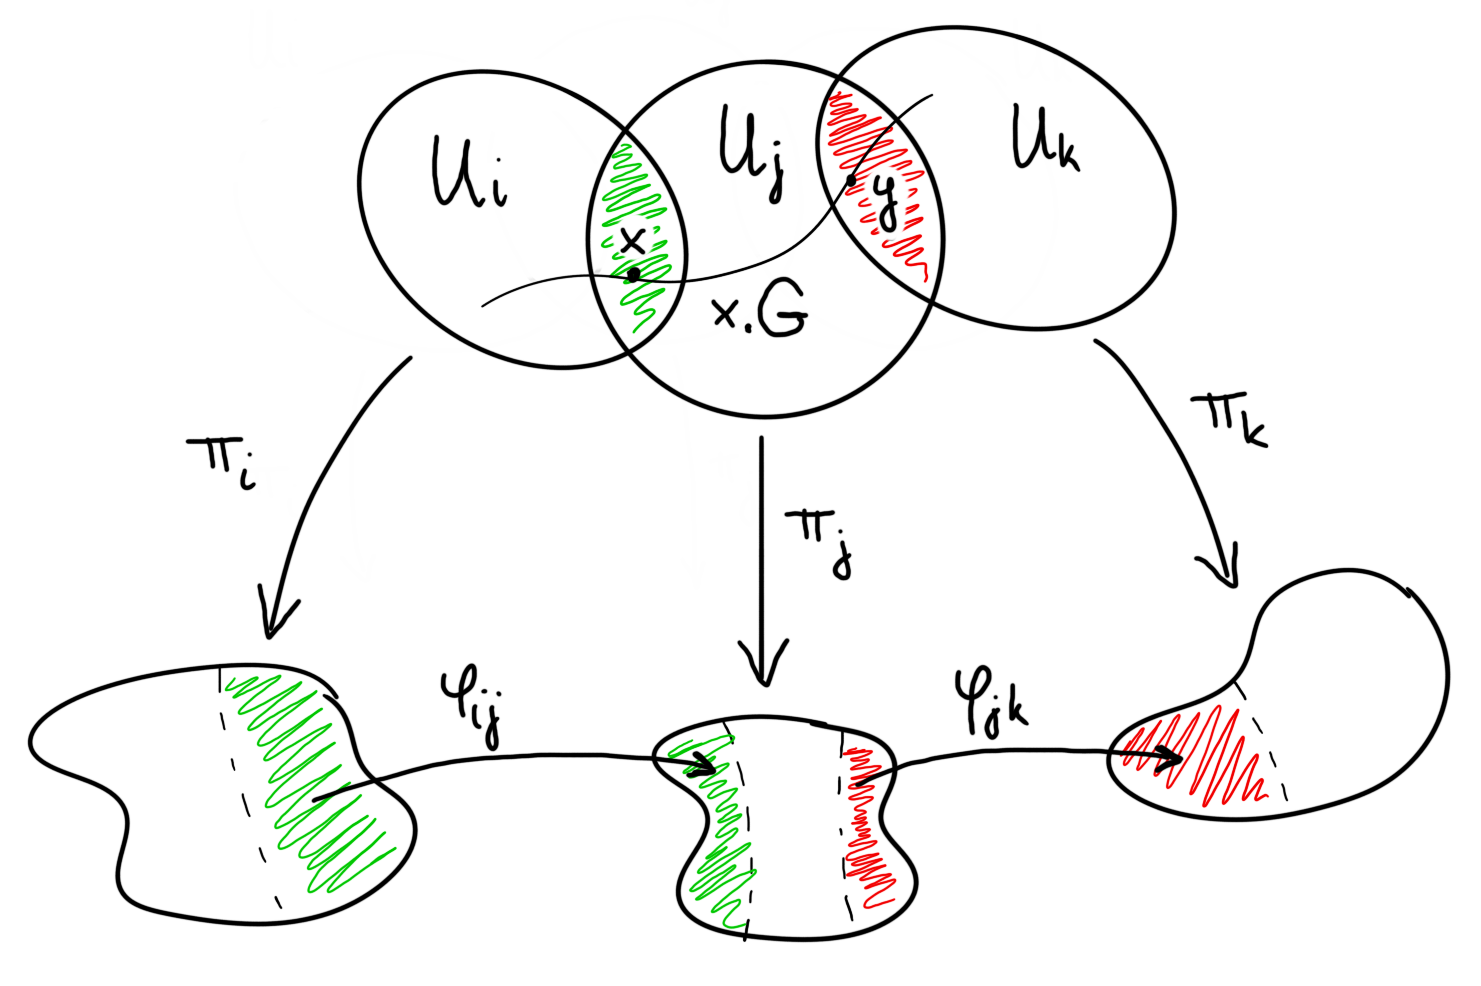
\includegraphics[scale=.9]{pictures/glueing.png}
    \end{figure}

    So in this case we do have $\pi_{j}(U_{i,j,k}) = \pi_{j}(U_{i,j}) \cap \pi_{j}(U_{j,k})$.
    And similarly $\pi_{i}(U_{i,j}) \cap \pi_{i}(U_{i,k}) = \pi_{i}(U_{i,j,k})$, so we need to show that $\varphi_{i,j}(\pi_{i}(U_{i,j,k})) = \pi_{j}(U_{i,j,k})$.
    But by construction we have $\varphi_{i,j} \circ \pi_{i,j} = \pi_{j,i}$, and this implies the desired equality.
    Hence $\varphi_{i,k}|_{\pi_{i}(U_{i,j,k})}$ and $\varphi_{j,k} \circ \varphi_{i,j}|_{\pi_{i}(U_{i,j,k})}$ are two isomorphisms between $\pi_{i}(U_{i,j,k})$ and $\pi_{k}(U_{i,k}) \cap \pi_{k}(U_{i,j}) = \pi_{k}(U_{i,j,k})$.
    But the corestriction of each $\pi_{i}$ to $\pi_{i}(U_{i,j,k})$ is also a geometric quotient of $U_{i,j,k}$ by $G$, so there exist unique isomorphisms $\psi_{i,k} \colon \pi_{i}(U_{i,j,k}) \cong \pi_{k}(U_{i,j,k})$ under $U_{i,j,k}$.
    In particular, since $\varphi_{i,k}|_{\pi_{i}(U_{i,j,k})}$ and $\varphi_{j,k} \circ \varphi_{i,j}|_{\pi_{i}(U_{i,j,k})}$ are two such isomorphisms, they must be equal, as we wanted to show.
    Hence the cocycle condition is satisfied and we may glue the $\pi_{i}$ together to obtain a $\mathbb{C}$-scheme morphism $\pi \colon X \to Z$ for some $\mathbb{C}$-scheme $Z$ obtained by glueing the $U_{i}/G$ together \cite[Exercise II.2.12]{har77}.
    Finally, since being a geometric quotient is local on the target, it suffices to show that this resulting morphism $\pi \colon X \to Z$ is a geometric quotient on an open cover of $Z$.
    But by construction $Z$ has an open cover $\{ V_{i} \}_{i \in I}$ in which each $V_{i}$ is identified with $U_{i}/G$ in such a way that the corresponding corestriction $\pi|_{\pi^{-1}(V_{i})} \colon \pi^{-1}(V_{i}) \to V_{i}$ is identified with the geometric quotient $\pi_{i} \colon U_{i} \to U_{i}/G$, so we are done.
  \end{proof}
\end{lm}

\begin{lm}\label{lm:avoidpoints}
  Let $X$ be a quasi-projective $\mathbb{C}$-scheme and let $x_{1},\ldots, x_{m} \in X$ be finitely many closed points.
  Then there exists an affine open subset $U \subseteq X$ such that $x_{i} \in U$ for all $i \in \{ 1, \ldots, m\}$.
  \begin{proof}
    We reproduce here the argument given in the notes that we are following most of the time, cited above.
    We regard $X$ as a locally closed subset of some $\mathbb{P}^{n}$.
    Then we look at its Zariski closure $\bar{X}$.
    If we find a hypersurface $H \subseteq \mathbb{P}^{n}$ which contains $\bar{X} \setminus X$ but not $x_{1}, \ldots, x_{m}$, then we are done, because $\mathbb{P}^{n} \setminus H$ is affine\footnote{If $H$ is a hyperplane, then $\mathbb{P}^{n} \setminus H \cong \mathbb{A}^{n}$.
    If $H$ is a hypersurface of degree $d$, then we may regard it as the intersection of a hyperplane with the image of $\mathbb{P}^{n}$ under the corresponding Veronese embedding, so the image of $\mathbb{P}^{n} \setminus H$ would be a closed subset inside the affine space given by the complement of this hyperplane, hence affine itself.} and $U := X \setminus H = \bar{X} \setminus H$ is closed inside an affine, hence affine itself.
    
    The main ingredient to find the hypersurface $H$ is the graded prime avoidance lemma \cite[\href{https://stacks.math.columbia.edu/tag/00JS}{Tag 00JS}]{stacks-project}.
    Let $\mathbb{C}[z_{0},\ldots,z_{n}]$ be the homogeneous coordinate ring of $\mathbb{P}^{n}$.
    If $\bar{X} = X$, we take $I$ to be $(z_{0}, \ldots, z_{n})$.
    Otherwise we take $I$ to be the homogeneous ideal of $\bar{X} \setminus X$.
    We take $\mathfrak{p}_{i}$ to be the maximal ideal corresponding to the point $x_{i}$ for each $i \in \{1, \ldots, m\}$.
    Let $i \in \{ 1, \ldots, m\}$.
    We have $(z_{0}, \ldots, z_{n}) \not\subset \mathfrak{p}_{i}$, because the maximal ideal $(z_{0}, \ldots, z_{n})$ does not correspond to any point in $\mathbb{P}^{n}$.
    And $x_{i} \not \in \bar{X} \setminus X$, because $x_{i} \in X$ by assumption.
    So in any case we have $I \not \subset \mathfrak{p}_{i}$.
    Hence we may apply graded prime avoidance to deduce the existence of a homogeneous polynomial of positive degree $f \in I$ which is not in any of the $\mathfrak{p}_{i}$, i.e.~such that $x_{i}$ is not in the hypersurface defined by $f$ for any $i \in \{1, \ldots, m\}$.
  \end{proof}
\end{lm}

\begin{thm}\label{thm:quotient}
  Let $\sigma \colon X \times G \to X$ be an action of a finite group on a quasi-projective $\mathbb{C}$-scheme.
  Then the geometric quotient $\pi \colon X \to X/G$ of $X$ by $G$ exists.
  The resulting $\mathbb{C}$-scheme $X/G$ is separated and of finite type over $\mathbb{C}$.
  Moreover, let $\mathbf{P}$ be any of the following properties:
  \begin{enumerate}[label=(\alph*)]
    \item irreducible,
    \item reduced,
    \item integral,
    \item normal,
    \item affine,
    \item projective.
  \end{enumerate}
  If $X$ has $\mathbf{P}$, then $X/G$ has $\mathbf{P}$.
  In particular, if $X$ is a (projective) variety, then $X/G$ is a (projective) variety.

  \begin{proof}
    We start by checking the existence of the geometric quotient with \Cref{lm:affinecover}.
    Since $X$ is quasi-projective over $\mathbb{C}$, it is also of finite type over $\mathbb{C}$, so it remains to find a $G$-invariant affine open cover of $X$.
    The orbit of every closed point $x \in X$ is contained in some affine open subset $U_{x}$ by \Cref{lm:avoidpoints}.
    It may be the case that $U_{x}$ is not yet $G$-invariant, but in any case the open neighborhood $\cap_{g \in G} U_{x}\cdot g$ of $x$ is $G$-invariant.
    Since $X$ is quasi-projective over $\mathbb{C}$, it is also separated, so the intersection of finitely many affine open subsets is again an affine open subset.
    Therefore we are able to find a $G$-invariant affine open neighborhood around each closed point of $X$, and by \Cref{lm:affinecover} the geometric quotient $\pi \colon X \to X/G$ of $X$ by $G$ exists.

    We show next separatedness of $X/G$ over $\mathbb{C}$.
    Note that $\pi \colon X \to X/G$ is finite and surjective, because we may check these properties on an open cover of the target and by construction of $X/G$ we may then assume that we are in the situation of \Cref{lm:finitesurjective}.
    We can then apply \cite[\href{https://stacks.math.columbia.edu/tag/09MQ}{Tag 09MQ}]{stacks-project} to deduce separatedness of $X/G$ over $\mathbb{C}$.

    The construction of $X/G$ combined with \Cref{lm:finitetype} shows that $X/G$ is locally of finite type over $\mathbb{C}$, and since $X$ is quasi-compact and $\pi$ is surjective, so is $X/G$.
    Hence $X/G$ is of finite type over $\mathbb{C}$.
    
    About the remaining properties $\mathbf{P}$ in the statement:
    \begin{enumerate}[label=(\alph*)]
      \item Since $\pi$ is surjective, so $X/G$ is irreducible as soon as $X$ is.
      \item Reducedness can be checked locally on $X/G$, so by construction of $X/G$ we may assume that we are in the situation of \Cref{cor:affinequotient}.
        But the corresponding ring morphism $A^{G} \to A$ is just the inclusion, so $A^{G}$ is reduced as soon as $A$ is reduced.
      \item The same argument as for reducedness applies, or one can also argue using that being integral is equivalent to being reduced and irreducible.
      \item Normality can again be checked locally on $X/G$, so we may assume that we are in the situation of \Cref{cor:affinequotient}.
        We need to show that $A^{G}$ is an integrally closed domain if $A$ is an integrally closed domain.
        For this we use compatibility of taking $G$-invariant subrings with localization \cite[Exercise 5.12]{am69}.
        Let $f \in (A^{G})_{(0)} = (A_{(0)})^{G}$ be a $G$-invariant element in the field of fractions of $A^{G}$, which is the subfield of $G$-invariant elements of the field of fractions of $A$.
        Suppose that $f$ is integral over $A^{G}$, i.e.~supposet that $f$ is the root of some monic polynomial with coefficients in $A^{G}$.
        We regard this monic polynomial as a monic polynomial with coefficients in $A$, which shows that $f$ is an element of $A_{(0)}$ which is integral over $A$.
        Since $A$ is integrally closed, this element of $A_{(0)}$ must already be in $A$.
        And it is $G$-invariant as well, so $f \in A^{G}$.
      \item If $X$ is affine, then we may apply \Cref{cor:affinequotient} directly to conclude that $X/G$ is affine as well.
      \item Properness of $X/G$ over $\mathbb{C}$ follows from the things that we have shown already, since the image of a proper scheme in a separated scheme of finite type is proper \cite[\href{https://stacks.math.columbia.edu/tag/03GN}{Tag 03GN}]{stacks-project}.
        An argument for the projectivity, which in fact shows that $X/G$ is quasi-projective as soon as $X$ is, can be found in \cite[Proposition IV.1.5]{knu71}.
        Projectivity would also follow from the GIT machinery, but we were intentionally trying to avoid getting into that here.
    \end{enumerate}
  \end{proof}
\end{thm}

\bibliographystyle{alpha}
\bibliography{main}
\vfill

\end{document}
